\section{Enunciado}

\hspace{1.27cm} En la \hyperref[fig1]{Figura 1} se muestra un estanque que se utiliza para monitoreo de especies marinas
endémicas de la Isla del Coco, donde se tiene un tanque cilíndrico vertical abierto en su
parte superior a la atmósfera, del cual se desea controlar el nivel del tanque manipulando
el caudal de entrada $Q_e$ ante posibles perturbaciones en el caudal de salida $Q_s$.

\begin{figure}[!h]
    \centering
    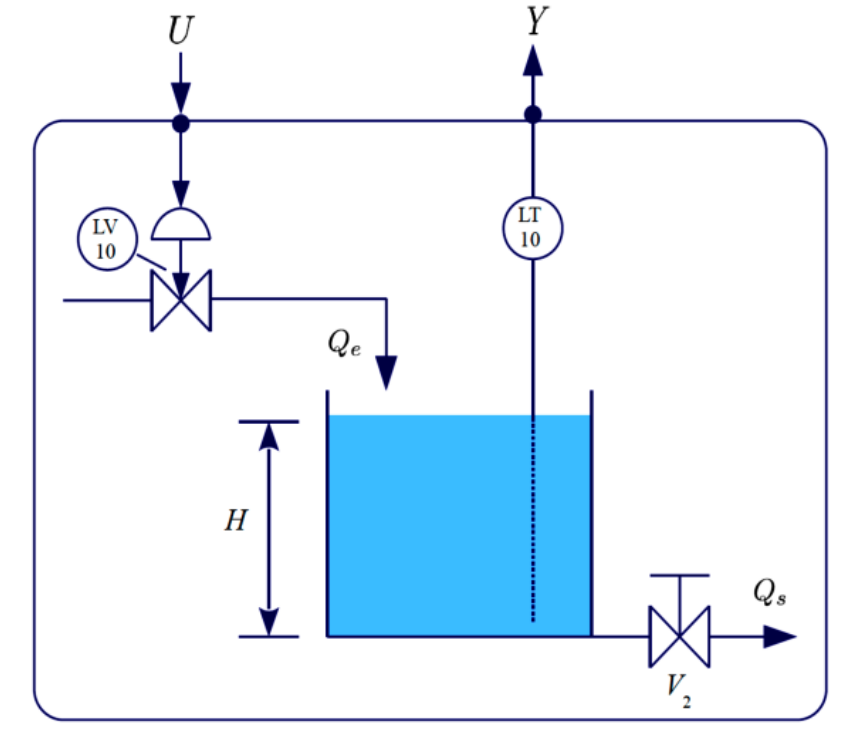
\includegraphics[width = 0.4\linewidth]{figs/fig1.png}
    \caption{Proceso Control de Nivel}
    \label{fig1}
\end{figure}

El modelo dinámico del proceso es:
\begin{align*}
    A\dv{H(t)}{t} = Q_e(t) -Q_s(t) = Q_e(t) - X _{vs} (t) K _{vs} \sqrt{\rho g H(t)}\numberthis\label{eq1}
\end{align*}
La característica estática es:
\begin{align*}
    H(t) = F (Q_e, X _{vs}) = \frac{1}{\rho g} \left( \frac{Q_e(t)}{X _{vs} (t) K _{vs}} \right) ^{2}\numberthis\label{eq2}
\end{align*}

El modelo linealizado es:
\begingroup 
\addtolength\jot{6pt} 
\begin{align*}
    h (s) = \frac{K _{1}}{ Ts + 1} q _{e} (s) &+ \frac{K _{2}}{Ts + 1} x _{vs} (s)\\
    K _{1} = \frac{2}{X _{vs0} K _{vs}} \sqrt{ \frac{H_0}{\rho g}}, \quad K _{2} =& - \frac{2 H_0}{X _{vs0}}, \quad T = \frac{2A}{X _{vs0} K _{vs}} \sqrt{ \frac{H_0}{\rho g}} \numberthis\label{eq3}
\end{align*}

\newpage
En donde:

\begin{figure}[!h]
    \centering
    \setlength\extrarowheight{3mm}
    \begin{tabular}{>{\centering\arraybackslash}p{5cm}p{5cm}>{\centering\arraybackslash}p{5cm}}
        \toprule\\[-2.5em]
        Variable/Parámetro & Descripción & Valor nominal\\
        \midrule
        $A$ & área transversal del tanque & \SI{5}{\metre\squared}\\
        $g$ & aceleración de la gravedad & \SI{9.81}{\metre\per\second\squared}\\
        $H$ & nivel de líquido en el tanque & [2.24 \textbf{2.5} 2.95] m\\
            & Altura máxima del tanque & \SI{3.6}{m}\\
            & Ámbito de medición del sensor & \SI{0}{m} -- \SI{3.25}{m} \\
        $Q _{e}$ & caudal de líquido de entrada & -- \\
        $Q _{s}$ & caudal de líquido de salida & -- \\
        $K _{vs}$ & constante de la válvula de salida del tanque & 0.001 \\
        $X _{vs}$ & apertura de la válvula de salida del tanque & \{0.4 \textbf{0.5} 0.6\} \\
        $\rho$ & densidad del líquido (agua de mar) & \SI{1027}{kg/\metre\cubed} \\
        $t$ & tiempo & s \\
        \bottomrule
    \end{tabular}
    \captionof{table}{Variables y parámetros del proceso control de nivel}
    \label{t1}
\end{figure}

\newpage

Para este sistema:

\begin{enumerate}[label=\alph*)]
    \item (5 puntos) Demuestre la obtención de la ecuación en el tiempo del modelo linealizado a
partir del modelo dinámico del sistema, utilizando el procedimiento algebraico de
linealización visto en clase, y a partir del mismo demuestre la obtención de las
respectivas funciones de transferencia.

\textit{Solución.} Para obtener el modelo linealizado, considere primero el vector de estados \\$ \textbf{x} = [H(t)]$ y el vector de entradas $ \textbf{u} = [Q_e(t),\,Xvs(t)] ^{T}$.
Al evaluar la \hyperref[eq2]{característica estática} en el punto de operación $ \textbf{x} _{0},\, \textbf{u} _{0}$, se busca $Q _{e,\,0}$. Note que $H _{0} = \SI{2.5}{m}$ y $X _{vs,\,0} = 0.5$ \label{po} se obtienen directamente del \hyperref[t1]{Cuadro 1}.
\begin{align*}
    H _{0} &= F (Q _{e,\,0},\,X _{vs,\,0})\\
           &= \frac{1}{\rho g} \left( \frac{Q _{e,\,0}}{X _{vs,\,0}K _{vs}} \right) ^{2}\\
    \frac{Q _{e,\,0}}{X _{vs,\,0} K _{vs}} &= \pm \sqrt{\rho g H _{0}}
    \intertext{Note que la cantidad en el lado izquierdo de la ecuación siempre es positiva, ya que $Q _{e,\,0}$ se refiere al caudal \textbf{entrante} y no saliente, $X _{vs} \in [0.4,\,0.6]$ y $K _{vs} = 0.001$, según el \hyperref[t1]{Cuadro 1}. Por tanto:}
    Q _{e,\,0} &= X _{vs,\,0} K _{vs} \sqrt{\rho g H _{0}}\\
    Q _{e,\,0} &= \SI{0.07953}{\metre\cubed\per\second}
\end{align*}

A partir del valor anterior y \hyperref[po]{el resto de valores}, el punto de operación del proceso viene dado por los vectores:
\begin{align*}
   \textbf{x}_{0}= \begin{bmatrix}
                        \SI{2.5}{m}
                    \end{bmatrix} 
                    \quad 
    \textbf{u}_{0}= \begin{bmatrix}
                        \SI{0.07953}{\metre\cubed\per\second}\\
                        0.5
                    \end{bmatrix}\numberthis\label{eq5}
\end{align*}


\end{enumerate}

Utilizando la plantilla \texttt{Tarea\_1.m} de MATLAB disponible en mediación virtual, calcule 

\begin{enumerate}[label=\alph*), start=2]
    \item (5 puntos) La ganancia del transmisor de nivel $K_t$. (\SI{}{\%\metre\tothe{-1}}) de forma que la señal
realimentada esté normalizada de 0 a 100\%.

\textit{Solución.} Según el \hyperref[t1]{Cuadro 1}, el sensor posee un ámbito de medición de $ \SI{0}{m} -- \SI{3.25}{m}$. Considerando que el sensor está en cascada con el transmisor, la máxima señal realimentada corresponderá a un valor $y _{max} = \SI{3.25}{m}$. A partir de este valor se normaliza la señal realimentada en el rango 0\% -- 100\%, tal que:
\begin{align*}
    K _{t}  &= \frac{100\%}{y _{max}}\\
    \Aboxed{K _{t}&= \SI{30.7692}{\percent\per\metre}}
\end{align*}



    \item (5 puntos) La constante de la válvula $K _{VC}$ (\SI{}{\metre\cubed\second\tothe{-1}\%\tothe{-1}}) de forma que la acción de control esté normalizada de 0\% a 100\%.

\textit{Solución.} Debido a que la variable manipulada es el caudal de entrada $Q _{e}(t)$, se debe diseñar la constante de la válvula $K _{VC}$ en función de su valor máximo $Q _{e,\,max}$ para que la acción de control esté acotada en el rango de 0\% -- 100\%. Dicho valor debe ser encontrado a partir de la característica estática. Evaluando la ecuación \hyperref[qe]{4} en $Q _{e,\,max}$, dicho valor se obtendrá cuando el nivel del tanque $H (t)$ y la apertura de la válvula de salida del tanque $X _{vs} (t)$ sean máximos. Según el \hyperref[t1]{Cuadro 1}, $H _{max} = \SI{2.95}{m}$ y $X _{vs,\,max} = 0.6$, por tanto:
\begin{align*}
    Q _{e,\,max} &= X _{vs,\,max} K _{vs} \sqrt{\rho g H _{max}}\\
    Q _{e,\,max} &= \SI{0.1034}{\metre\cubed\per\second}
\end{align*}
Y por tanto, la constante de la válvula $K _{VC}$ vendrá dada por:
\begin{align*}
    K _{VC} &= \frac{Q _{e,\,max}}{100\%}\\
    \Aboxed{K _{VC} &= \SI{0.001034}{\metre\cubed\per\second\per\percent}}
\end{align*}



    \item (20 puntos) Implemente el sistema real en Simulink utilizando la ecuación del modelo
        dinámico del proceso tal como se observa en la \hyperref[fig2]{Figura 2}. \textbf{Debe indicar la condición inicial ($H_0$) en los parámetros del bloque Integrador.}
\textit{Solución.} Se implementó el sistema real en Simulink por medio de la ecuación del \hyperref[eq1]{modelo dinámico del proceso}. A continuación se muestra el diagrama de bloques que se obtuvo:

\begin{figure}[!h]
    \centering
    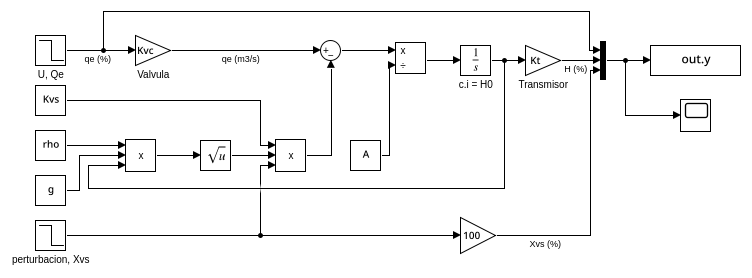
\includegraphics[width = 0.8\linewidth]{figs/fig2.png}
    \caption{Diagrama de bloques del sistema real implementado en Simulink}
    \label{fig2}
\end{figure}


    \item (15 puntos) Calcule el valor de $T$, $K_1$, $K_2$ del modelo linealizado. Implemente el diagrama de bloques en Simulink del sistema tal como se observa en la Figura 3.
\textit{Solución.} A partir de los \hyperref[eq3]{parámetros del modelo linealizado} y los datos del \hyperref[t1]{Cuadro 1}, se obtienen sus valores numéricos a continuación:

\begin{alignat*}{2}
    T &= \frac{2A}{X _{vs0} K _{vs}} \sqrt{ \frac{H_0}{\rho g}} &&= \SI{315.0506}{s}\\
    K _{1} &= \frac{2}{X _{vs0} K _{vs}} \sqrt{ \frac{H_0}{\rho g}} &&= \SI{63.0101}{\second\per\metre\squared}\\
    K _{2} &= - \frac{2 H_0}{X _{vs0}} &&= \SI{-10}{m}
\end{alignat*}

\newpage

Se implementó el siguiente diagrama de bloques en Simulink.

\begin{figure}[!h]
    \centering
    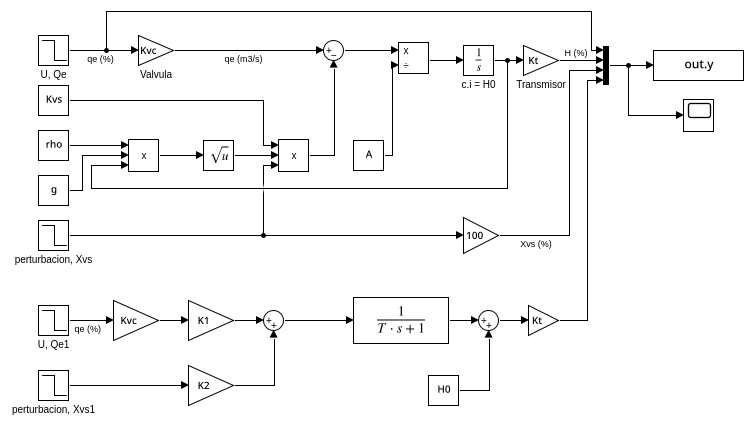
\includegraphics[width = 0.6\linewidth]{figs/fig3.png}
    \caption{Diagrama de bloques del sistema real y linealizado}
    \label{fig3}
\end{figure}

    \item (20 puntos) Obtenga la respuesta del sistema (obtenida en el punto c) y compárela con la del sistema linealizado (obtenida en el punto d) \textbf{en una misma gráfica} utilizando Simulink/MATLAB, cuando ambos se encuentran en el punto de operación más probable y se producen los siguientes cambios:
\textit{Solución.} Se obtuvieron las siguientes respuestas para el sistema linealizado $H _{linealizado}(t)$ y el sistema real $H _{real}(t)$ ante los cambios especificados en el enunciado.

\begin{figure}[!h]
    \centering
    \begin{minipage}{0.5\linewidth}
        \centering
        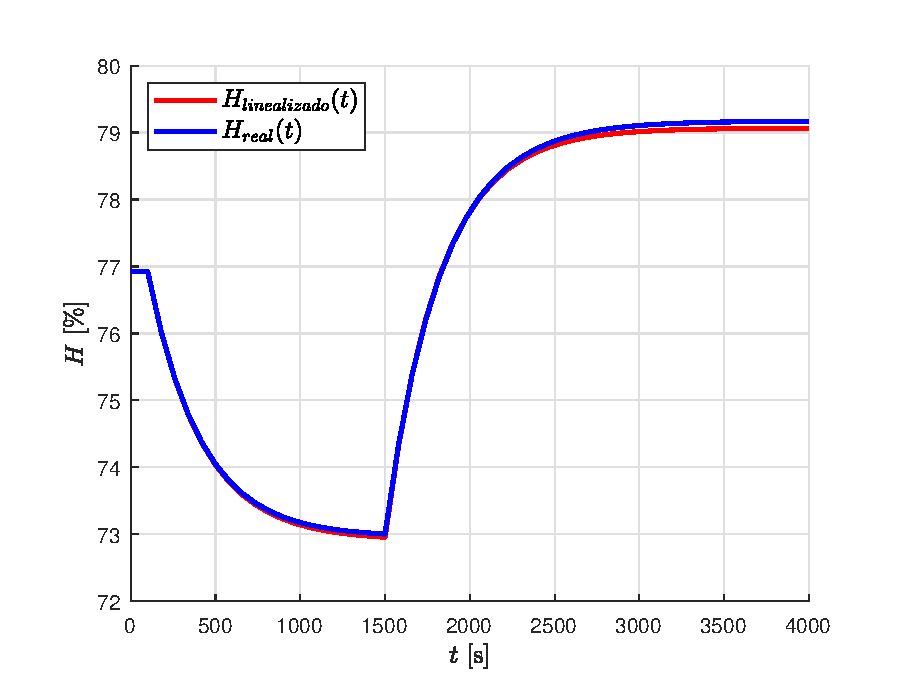
\includegraphics[width = 0.8\linewidth]{figs/fig4.eps}
        \caption*{(a): $\Delta U = -2\% \quad \Delta D = -0.02$}
    \end{minipage}%
    \begin{minipage}{0.5\linewidth}
        \centering
        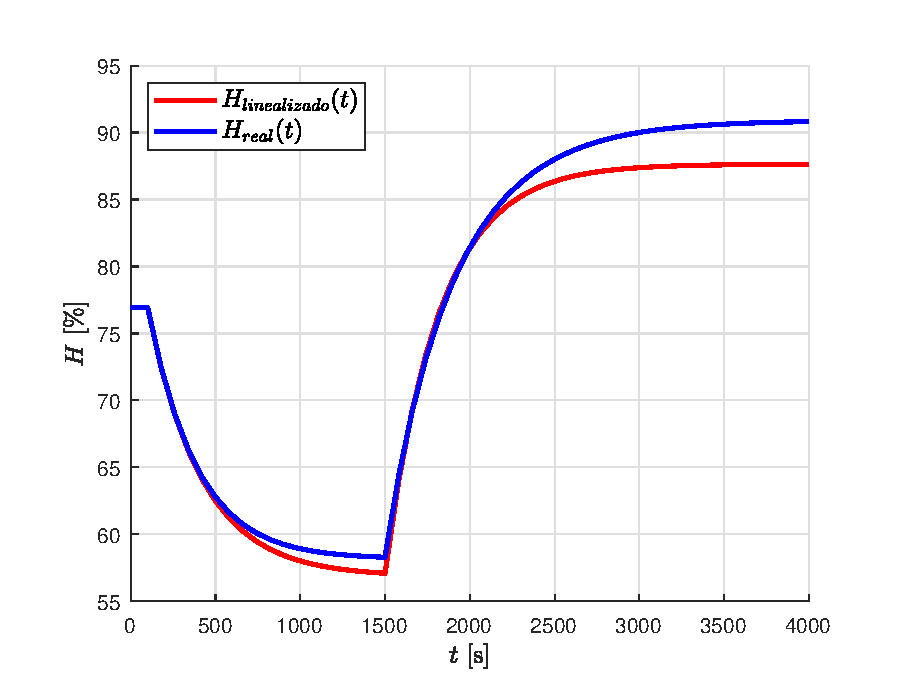
\includegraphics[width = 0.8\linewidth]{figs/fig5.eps}
        \caption*{(a): $\Delta U = -10\% \quad \Delta D = -0.1$}
    \end{minipage}
    \caption{Respuesta del sistema real y linealizado, ante distintas señales de control y perturbaciones.}
    \label{fig4}
\end{figure}
\newpage

        \begin{enumerate}[label=\roman*.]
            \item Un cambio escalón en la señal de control de $\Delta U = -2\%$, seguido de un cambio escalón en la perturbación de $\Delta D = -0.02$.
                Considere que el sistema debe estabilizarse antes de aplicar el segundo cambio escalón.
            \item Un cambio escalón de la señal de control de $\Delta U = -10\%$, seguido de un cambio escalón en la perturbación de $\Delta D = -0.1$. Considere que el sistema debe estabilizarse antes de aplicar el segundo cambio escalón.
        \end{enumerate}
        Indique las gráficas en su solución y adjunte el archivo \texttt{.slx}.
    \item (20 puntos) A partir de la ecuación de la característica estática obtenga utilizando MATLAB
y en una misma figura, la curva estática del proceso para los tres posibles valores de la
apertura de la válvula de salida. Muestra la relación entre $m(t)$ y $c(t)$. 
\textit{Solución.} A continuación, se muestran las curvas obtenidas a partir de la ecuación característica para distintos valores de la perturbación $X _{vs} (t)$.

\begin{figure}[!h]
    \centering
    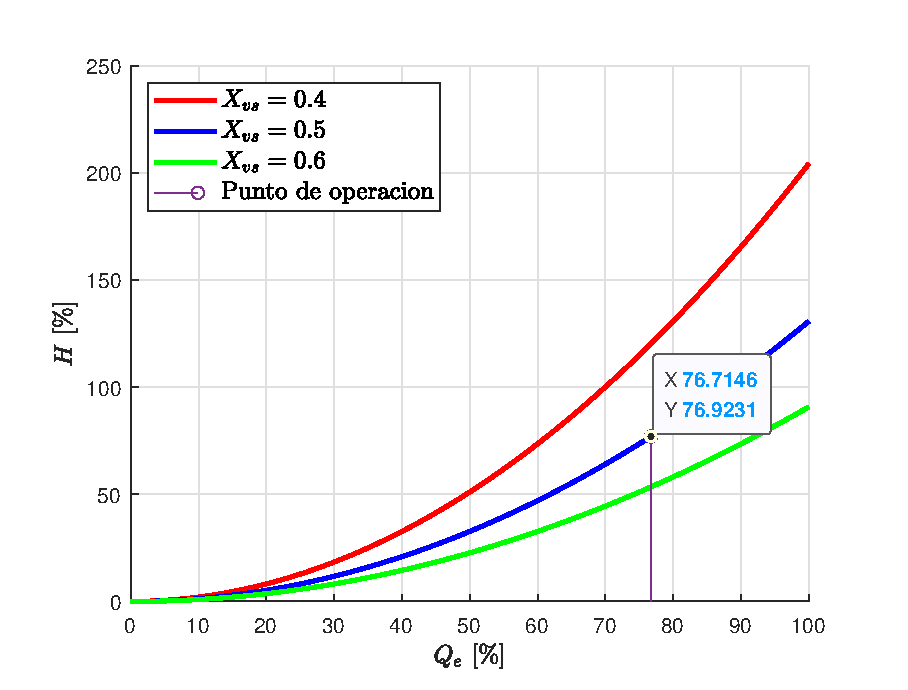
\includegraphics[width = 0.5\linewidth]{figs/fig6.eps}
    \caption{Curva estática del proceso para los distintos valores del pocentaje de apertura de la válvula de salida $X _{vs} (t)$}
    \label{fig5}
\end{figure}

Note que el punto de operación se encuentra en el valor central de $X _{vs} (t)$, ya que este fue el valor que se tomó en cuenta para el cálculo del punto de operación, así como para generar el modelo linealizado.


\textbf{Indique en la figura el punto de operación más probable del sistema}. Presente la gráfica en su solución y comente sobre la forma de las curvas.
    \item (10 puntos) A partir de los resultados anteriores, observe la respuesta del nivel ante los
cambios en el caudal de entrada y la apertura de la válvula de salida, ¿son razonables?
Comente sobre la validez del modelo lineal cuando se producen cambios en el punto
de operación del sistema.
\textit{Solución.} Los resultados que se muestran en la \hyperref[fig4]{Figura 4} y la \hyperref[fig5]{Figura 5} son razonables, ya que el modelo linealizado logra aproximar efectivamente el proceso no lineal cuando el punto de operación varía ligeramente. Esto es debido a que la linealización se realiza por medio de series de Taylor, las cuales son conocidas por únicamente ser aproximaciones válidas a funciones matemáticas cuando se evalúa la función cerca del centro de la serie. Esto es claro al comparar las subfiguras (a) y (b) en la \hyperref[fig4]{Figura 4}, ya que en la figura (b) el modelo linealizado se desvía más del modelo real en comparación a la figura (a). siendo la causa principal un cambio más significativo en el punto de operación.


\vspace{1em}
\begin{mdframed}
        Así como el código fuente que genera este reporte y el código de MATLAB para generar las gráficas mostradas anteriormente se encuentran en el siguiente repositorio de Github:
    
    \begin{center}
        \href{https://github.com/Roger-505/tareas-ie0431}{\texttt{https://github.com/Roger-505/tareas-ie0431}}
    \end{center}
\end{mdframed}

\end{enumerate}

